\section{引言}
\label{sec:intro}

在 GPU 上实现深度神经网络（DNN）的高性能执行，对于现代机器学习应用至关重要。
当今的 DNN 框架通常使用张量程序来描述 DNN 计算，张量程序是有向无环图，其节点和边分别表示张量代数运算符（如矩阵乘法）以及运算符之间共享的张量（即 $n$ 维数组）。

为了优化输入的张量程序，现有框架（如 PyTorch~\cite{pytorch} 和 TensorFlow~\cite{Tensorflow}）使用手动设计的规则将张量程序映射到专家编写的 GPU 核。
这些方法通常需要大量工程工作来设计和实现优化规则，并且可能会错过某些优化机会。
为了应对这些挑战，近年来的研究引入了{\em 自动化}方法，通过搜索涵盖广泛的程序变换空间并根据目标 GPU 上的实际性能来应用变换，从而优化张量程序。
这些方法大体可分为两类。

第一类工作，包括 Halide~\cite{halide}、TVM~\cite{tvm} 和 Ansor~\cite{ansor}，其出发点是 Halide 中引入的算法与调度分离思想\footnote{在调度优化文献中，算法（algorithm）描述了核中需要计算什么，而调度（schedule）规定了如何执行这个核。}，在固定算法的前提下优化张量程序的{\em 调度}。
对于给定的算法，这些优化器通过搜索在目标硬件上执行核的可能策略，自动生成高性能核。
然而，由于 DNN 的线性代数本质，张量程序可以用数学上等价的多种算法来表示。现有的基于调度的优化器只考虑算法由用户手工指定的核，从而错失了优化机会。

第二类工作，包括 TASO、Grappler、Tensat 和 PET，考虑{\em 代数变换}，即利用张量程序不同算法之间的数学等价性~\cite{TASO, tensorflow_grappler, yang2021equality, wang2021pet}。
代数变换的示例包括：（1）将一种线性代数运算符转换为另一种，例如将卷积变换为矩阵乘法；（2）融合多个运算符以减少内存访问和核启动开销；以及（3）根据交换律、结合律和分配律重新组织运算符。
这些优化器在算法层面执行代数变换，并要求程序员手动指定可用运算符及其实现。
因此，它们受限于所提供核的性能。

所有现有的自动化优化方法，无论来自哪一类，都仍然要求程序员手动指定一组核（每个核由一个张量函数定义），然后探索代数变换{\em 或}调度变换的搜索空间。
然而，一些先进的性能优化需要在 GPU 计算层次的核、线程块和线程三个层次上协同进行变换，甚至涉及引入全新的核计算（例如，一个能分解标准核并只融合特定计算的自定义核）。
这类优化超出了现有自动化方法的搜索空间，至今仍需手动实现。

其中一个典型例子是 FlashAttention~\cite{dao2023flash}（详见 \S\ref{subsec:benchmark_results}），它通过在算法层面重排运算符（代数变换）、重组跨 GPU 核的计算（生成新的自定义核）以及调整每个核的并行化策略以适应 GPU 架构（调度变换），在 GPU 上优化了注意力~\cite{transformers} 的计算。
这个例子所需的变换无法被现有框架自动发现，必须手动实现。
FlashAttention 在 Triton~\cite{tillet2019triton}（一种广泛使用的张量程序优化器）中的实现，即便使用高级编程语言，也包含超过 700 行代码~\cite{triton-flashattention}。

我们提出 \sys，这是第一个面向张量程序的{\em 多层次超级优化器}。
\sys 能够自动发现并验证张量程序的复杂优化方案，这些方案需要联合优化代数变换、调度变换，并发现新的自定义核。

\sys 的核心思想是 \graphs——一种{\em 层次图表示}，能够在 GPU 计算层次的多个层次上描述张量程序。
通过统一处理核、线程块和线程这三个层次，\graphs 能够在这些层次上捕获代数变换和调度变换。
此外，优化 \graph 还可以引入新的自定义核，这超出了代数变换和调度变换的范畴。
例如，\sys 自动发现了代表 FlashAttention~\cite{dao2023flash} 及其推理变体 FlashDecoding~\cite{tri2023flashdecoding} 的 \graphs，以及在某些使用场景中超越这些手动设计的核最高达 $2.2\times$ 的其他 \graphs。
\sys 发现的大多数优化方案超出了现有方法的搜索空间。

\begin{figure}
    \centering
    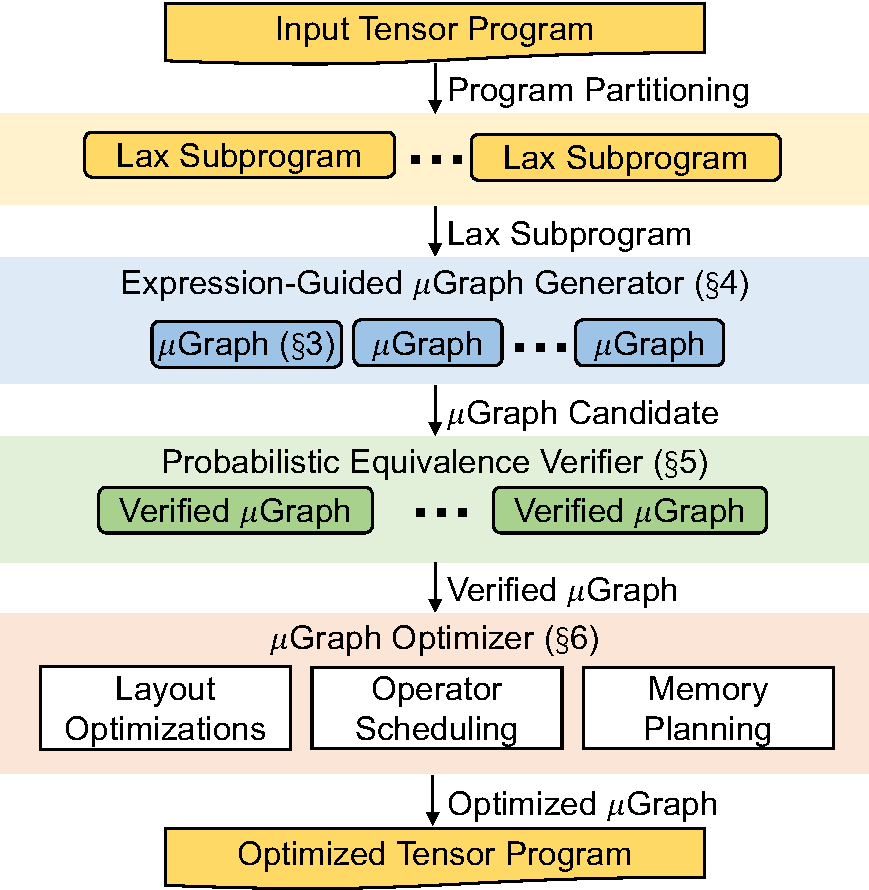
\includegraphics[scale=0.48]{figs/overview3-crop.pdf}
    \vspace{\captionvspace}
    \caption{\sys 系统概览。}
    \vspace{-1em}
    \label{fig:overview}
\end{figure}

\Cref{fig:overview} 展示了 \sys 的系统概览。
\sys 首先将输入的张量程序拆分为属于受限 \lax 片段的子程序。
\lax 片段在 \S\ref{sec:verify} 中有正式定义，包括多线性运算符（如矩阵乘法和卷积）、除法（用于归一化）以及有限的指数运算（用于激活函数）。
将张量程序划分为 \lax 子程序，能够在保留大多数优化机会的同时缩减每个子程序的优化搜索空间；同时还支持 \sys 的概率等价验证器。

\paragraph{表达式引导的 \graph 生成器。}
对于每个 \lax 子程序，\sys 的{\em 表达式引导生成器}穷举搜索与之等价的所有可能 \graphs。
\sys 必须解决的一个关键挑战是，与先前的超级优化技术相比，其搜索空间要大得多。
例如，TASO~\cite{TASO} 和 PET~\cite{wang2021pet} 只在核层次上使用固定的预定义核集合搜索张量程序，而 \sys 则在核、线程块和线程三个层次上同时考虑超级优化。
为了高效导航这个更大的搜索空间，\sys 引入了一种基于{\em 抽象表达式}的新型剪枝技术，该技术在提供一定理论最优性保证的同时，大幅减少了 \sys 需要考察的 \graphs 数量。
\sys 通过将搜索重点放在核和块层次，并对线程层次采用基于规则的方法，进一步缩减了搜索空间。

\paragraph{概率等价验证器。}
对于 \sys 发现的 \graph，验证其与输入程序的功能等价性带来了另一个挑战，因为程序的输入和输出张量可能包含多达数百万个元素。
\sys 的核心思想是{\em 概率等价验证}，通过在有限域上执行随机测试来检验 \graphs 之间的等价性。
虽然随机测试通常对一般程序只能提供有限的正确性保证，但 \sys 利用一个新颖的理论结论证明：\lax 片段施加的限制确保了对于 \lax 程序，在有限域上的随机测试能够提供强有力的正确性保证。
具体而言，我们证明了多项式恒等测试（PIT）算法~\cite{schwartz1980fast, zippel1979probabilistic} 可以推广到 \lax 程序，从而得到一种可使精度任意高的 \lax 程序等价性随机算法。
\sys 使用这一随机算法来（概率性地）确保每个优化后的程序与输入程序等价。

\paragraph{\graph 优化器。}对于每个经过验证的 \graph，\sys 的{\em \graph 优化器}通过进一步考虑潜在的张量布局、调度运算符执行顺序，以及在核、线程块和线程三个层次上规划内存分配，来最大化其运行时性能。
最终，\sys 根据为每个 \lax 子程序找到的最佳 \graph，返回优化后的张量程序。

\paragraph{评估结果。}
我们在 NVIDIA A100 和 H100 GPU 上针对多种常用 DNN 基准测试评估了 \sys。
即使对于被现有系统广泛使用和深度优化的 DNN 基准（如用于大语言模型（LLM）的分组查询注意力~\cite{grattafiori2024llama3herdmodels}），\sys 通过利用现有系统中缺失的微妙自定义核和优化手段，仍能将现有方法的性能提升最高达 $3.3\times$。
